\documentclass[a4paper]{article}

\usepackage[utf8]{inputenc}
\usepackage[T1]{fontenc}
\usepackage{textcomp}
\usepackage[italian]{babel}
\usepackage{amsmath, amssymb}
\usepackage{siunitx}
\usepackage{caption}
\usepackage{graphicx}
\usepackage{subcaption}
\usepackage{booktabs} % Opzionale, per tabelle più belle se vuoi (\toprule, \midrule, \bottomrule)
\usepackage{ragged2e} % Per \Centering nelle minipage
\usepackage{float} % Per [htbp]
\usepackage{fullwidth}
\usepackage{darkmode}
%\enabledarkmode
\usepackage[margin=2cm]{geometry}

% ======================================================
% Impostazioni siunitx (opzionale, ma utile)
% ======================================================
\sisetup{
    output-decimal-marker = {,}, % Usa la virgola come separatore decimale
    uncertainty-mode = separate, % Mostra incertezza come ±
    separate-uncertainty = true, % Forza la separazione
    locale = IT, % Impostazioni locali italiane (es. per la virgola)
    group-digits = false, % Evita di raggruppare le cifre (es. 10000 vs 10 000)
    per-mode=symbol % usa / per le unità composte es. km/h
}

% ======================================================
% Appendice con le tabelle dati
% ======================================================
\usepackage{titling}
\usepackage{appendix}
\usepackage[colorlinks=true, linkcolor=blue, citecolor=blue, urlcolor=blue]{hyperref} % Per riferimenti cliccabili (opzionale ma utile)
\usepackage[italian,nameinlink]{cleveref} % Per riferimenti più intelligenti (\cref, \Cref)

\renewcommand{\appendixname}{Appendice} % Traduce "Appendix" in "Appendice"
\renewcommand{\appendixtocname}{Appendici} % Traduce "Appendices" nel ToC
\renewcommand{\appendixpagename}{Appendici} % Traduce "Appendices" nell'header/footer

% Configurazioni cleveref per l'italiano
\crefname{section}{sezione}{sezioni}
\Crefname{section}{Sezione}{Sezioni}
\crefname{table}{tabella}{tabelle}
\Crefname{table}{Tabella}{Tabelle}
\crefname{figure}{figura}{figure}
\Crefname{figure}{Figura}{Figure}
\crefname{equation}{equazione}{equazioni}
\Crefname{equation}{Equazione}{Equazioni}
\crefname{footnote}{nota}{note}
\Crefname{footnote}{Nota}{Note}


\title{Microonde}
\author{Alessio Ramirez, Michele Rota, Sofia Zocchi}
\date{Maggio 2025} % Modificato per coerenza linguistica

\begin{document}
\maketitle
\section{Caratterizzazione del fascio}
\subsection{Polarizzazione}
\subsubsection{Obiettivo}
Studiare la polarizzazione del fascio prodotto dall'emettitore e valutare la validità della Legge di Malus.

\subsubsection{Metodo}
Dal momento che l'emettitore produce un'onda polarizzata e il ricevitore si comporta come un filtro polarizzatore, è possibile osservare il segnale misurato al variare dell'angolo di cui è ruotato il ricevitore. Innanzitutto abbiamo disposto emettitore e ricevitore frontalmente, lungo lo stesso asse e a distanza fissata. Abbiamo quindi campionato, al variare di $\alpha$, angolo tra la direzione di polarizzazione dell'onda e l'asse di trasmissione del filtro, i valori di tensione restituiti dal voltmetro collegato al ricevitore. Lo studio della dipendenza del segnale da $\cos(\alpha)$ è fondamentale per valutare se quanto restituito dal ricevitore risulti proporzionale al campo elettrico o all'intensità dell'onda. In quest'ultimo caso si avrebbe la validità della Legge di Malus:
\begin{equation}
I = I_0 \cos^2(\alpha)
\label{eq:legge_di_Malus}
\end{equation}
Mentre, nel caso di una dipendenza da $|\cos(\alpha)|$, si avrebbe una legge della forma
\begin{equation}
V = V_0|\cos(\alpha)|
\label{eq:legge_modulo_coseno}
\end{equation}
Una volta raccolti i dati, ne abbiamo quindi valutato l'accordo con le relazioni~\eqref{eq:legge_di_Malus}~\eqref{eq:legge_modulo_coseno}.

\subsubsection{Dati}
Abbiamo raccolto i valori di tensione misurati in seguito ad una rotazione del ricevitore attorno al proprio asse di un angolo $\alpha$ compreso tra $\ang{0}$ e $\ang{180}$, ogni $\ang{5}$\footnote{Tutti gli angoli misurati in gradi sono stati poi convertiti in radianti.}. Abbiamo considerato come errore sul valore di $\alpha$ la sensibilità del goniometro montato sul ricevitore, che segnava gradi multipli di 5, dunque l'errore lo abbiamo assunto di 3 gradi, mentre, per quanto riguarda l'incertezza sul segnale, abbiamo osservato le fluttuazioni del valore di tensione restituito dal voltmetro. Sono stati così stimati errori variabili, differenti da misura a misura, e corrispondenti a metà dell'intervallo entro cui oscillavano i valori di tensione.
Quanto misurato è visibile nella \Cref{tab:dati_Malus}.
\begin{table}[htbp]
\centering
\begin{tabular}{|c|c|}
\hline
$\alpha$ & Tensione \\\hline\hline
0 ± 50 mrad & 2.97 ± 0.02 V \\
87 ± 50 mrad & 2.95 ± 0.02 V \\
175 ± 50 mrad & 2.90 ± 0.02 V \\
262 ± 50 mrad & 2.79 ± 0.01 V \\
349 ± 50 mrad & 2.67 ± 0.02 V \\
436 ± 50 mrad & 2.51 ± 0.02 V \\
524 ± 50 mrad & 2.33 ± 0.02 V \\
611 ± 50 mrad & 2.11 ± 0.01 V \\
698 ± 50 mrad & 1.92 ± 0.01 V \\
785 ± 50 mrad & 1.67 ± 0.02 V \\
873 ± 50 mrad & 1.42 ± 0.02 V \\
960 ± 50 mrad & 1.13 ± 0.01 V \\
1.05 ± 0.05 rad & 890 ± 10 mV \\
1.13 ± 0.05 rad & 580 ± 10 mV \\
1.22 ± 0.05 rad & 370 ± 10 mV \\
1.31 ± 0.05 rad & 190 ± 10 mV \\
1.40 ± 0.05 rad & 70 ± 10 mV \\
1.48 ± 0.05 rad & 20 ± 10 mV \\
1.57 ± 0.05 rad & 0 ± 10 mV \\
1.66 ± 0.05 rad & 30 ± 10 mV \\
1.75 ± 0.05 rad & 120 ± 10 mV \\
1.83 ± 0.05 rad & 270 ± 10 mV \\
1.92 ± 0.05 rad & 470 ± 10 mV \\
2.01 ± 0.05 rad & 720 ± 10 mV \\
2.09 ± 0.05 rad & 980 ± 10 mV \\
2.18 ± 0.05 rad & 1.26 ± 0.01 V \\
2.27 ± 0.05 rad & 1.52 ± 0.02 V \\
2.36 ± 0.05 rad & 1.75 ± 0.02 V \\
2.44 ± 0.05 rad & 2.00 ± 0.02 V \\
2.53 ± 0.05 rad & 2.24 ± 0.02 V \\
2.62 ± 0.05 rad & 2.45 ± 0.01 V \\
2.71 ± 0.05 rad & 2.65 ± 0.02 V \\
2.79 ± 0.05 rad & 2.81 ± 0.02 V \\
2.88 ± 0.05 rad & 2.89 ± 0.02 V \\
2.97 ± 0.05 rad & 2.93 ± 0.03 V \\
3.05 ± 0.05 rad & 2.96 ± 0.02 V \\
3.14 ± 0.05 rad & 2.97 ± 0.02 V \\
\hline
\end{tabular}
\caption{Dati sperimentali per la verifica della Legge di Malus.}
\label{tab:dati_Malus}
\end{table}

\subsubsection{Analisi dati}
\begin{figure}[htbp]
	\centering
	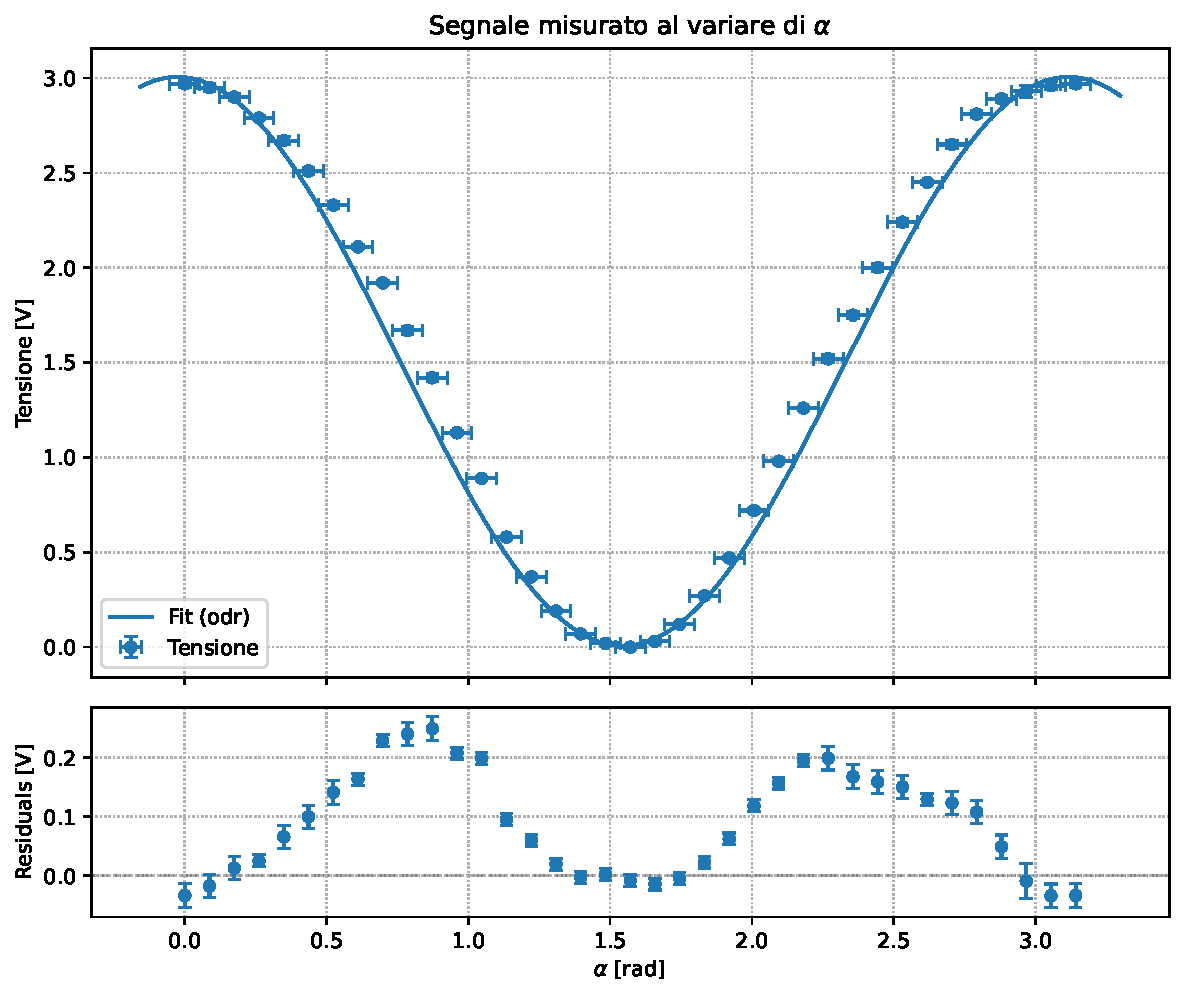
\includegraphics[width=0.7\textwidth]{grafici/Malus.pdf}
	\caption{Fit segnale al variare dell'inclinazione del filtro polarizzatore (Malus).}
	\label{fig:Malus_grafico}
\end{figure}

\begin{figure}[htbp]
	\centering
	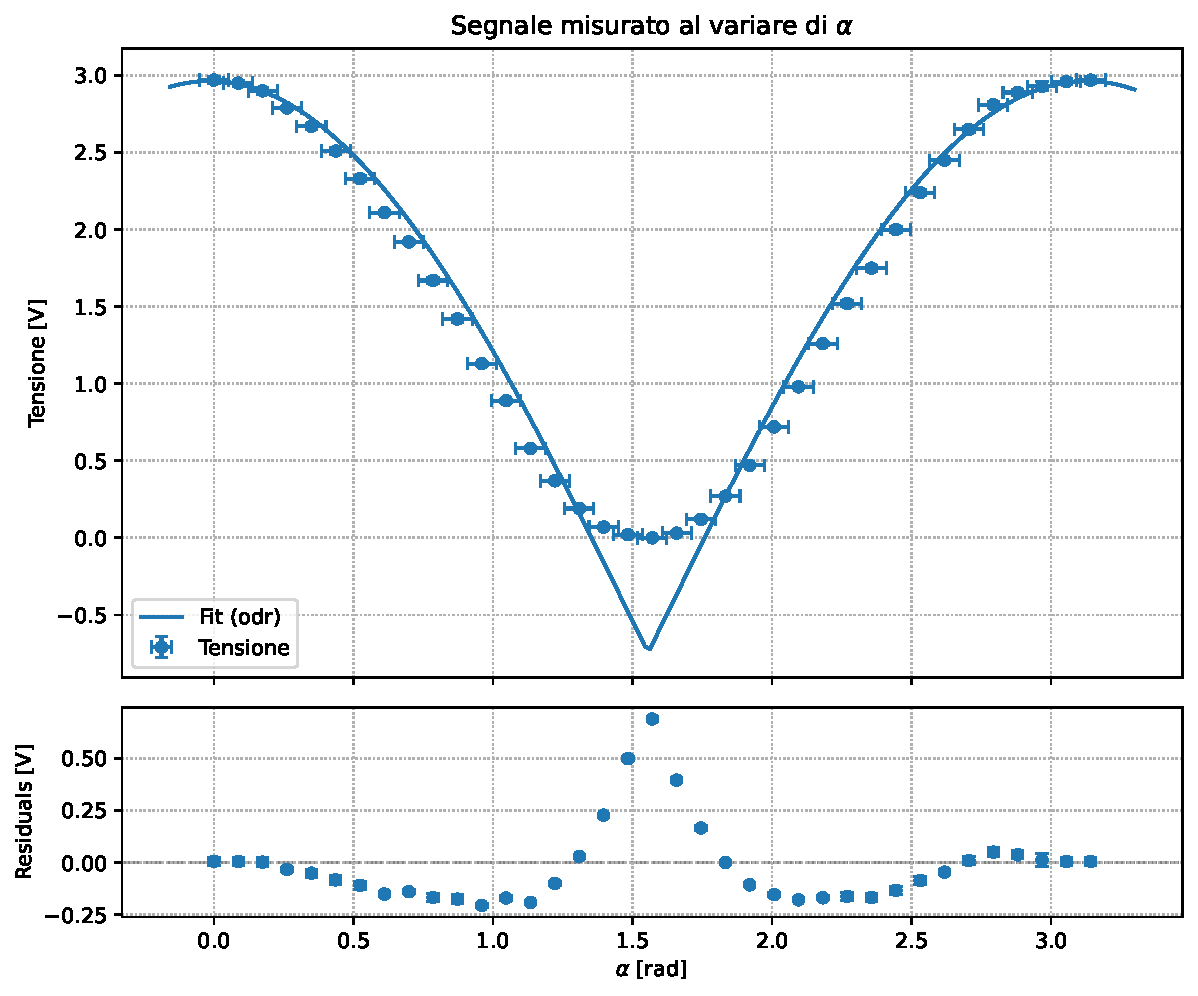
\includegraphics[width=0.7\textwidth]{grafici/abs_cos.pdf}
	\caption{Fit segnale al variare dell'inclinazione del filtro polarizzatore (|cos|).}
	\label{fig:modulo_coseno}
\end{figure}

Quanto misurato è stato utilizzato per verificare la validità della Legge di Malus. Abbiamo quindi effettuato un fit dei dati utilizzando una relazione della forma $V = k+V_0\cos^2(\alpha - \alpha_0)$, scelta sulla base di quanto descritto dalla \cref{eq:legge_di_Malus} e nell'ipotesi che il segnale di tensione fosse proporzionale all'intensità della radiazione. Nel realizzare l'interpolazione abbiamo considerato anche la presenza di un offset verticale $k$ e orizzontale $\alpha_0$, dal momento che la lettura fatta dal ricevitore non è riferita ad una scala assoluta, ma anzi poteva essere traslata o amplificata utilizzando le apposite manopole, e potrebbe esserci un errore sistematico nella misura dell'angolo del ricevitore, dal momento che non è detto che siano perfettamente parallele le direzioni di polarizzazione quando si misura $\alpha = 0$. I parametri dei fit ottenuti mediante interpolazione sono raccolti nella \Cref{tab:fit_Malus}; i loro andamenti sono visualizzabili nei grafici in \Cref{fig:Malus_grafico,fig:modulo_coseno}. Si noti inoltre che il ricevitore utilizzato non aveva una manopola per l'offset utilizzabile, e in assenza del segnale dell'emettitore prevaleva il rumore di fondo. Questo ci porta a introdurre un parametro di offset nelle interpolazione, che ci aspettiamo essere confrontabile con lo 0, ma senza un valore atteso realmente misurabile.
\begin{table}[htbp]
\centering
\begin{tabular}{|l|cccccc|}
\hline
Fit & k & $V_0$ & $\alpha_0$ & $\chi^2$ & DoF & $\chi^2/\nu$ \\\hline\hline
Fit Malus & 6.5 ± 8.8 mV & 2.999 ± 0.018 & -25.4 ± 9.1 m & 34.3 & 34 & 1.01 \\\hline
Fit $|\cos|$ & -746 ± 79 m & 3.710 ± 0.082 & -15 ± 11 m & 51.7 & 34 & 1.52 \\\hline
\end{tabular}
\caption{Risultati del fit per la Legge di Malus.}
\label{tab:fit_Malus}
\end{table}

\subsubsection{Conclusione}
Come si può osservare nella \Cref{tab:fit_Malus}, risulta compatibile un'interpolazione quadratica nel coseno, con un offset compatibile con 0, un $\alpha_0$ ragionevolmente piccolo, mentre la miglior interpolazione con il modulo del coseno risulta incompatibile\footnote{un $\chi^2/\nu$ di 1.5, con 34 gradi di libertà, risulta incompatibile con qualsiasi soglia ragionevole per il p-value}, con dei valori negativi che non possono rappresentare un fenomeno fisico reale. la Legge di Malus risulta verificata, così come l'ipotesi che il segnale misurato dipenda dall'intensità dell'onda, in quanto proporzionale a $\cos^2(\alpha)$.

\subsection{Ampiezza e geometria del fascio}

\subsubsection{Obiettivo}
L'obiettivo di questa parte dell'esperimento è caratterizzare l'ampiezza e la geometria del fascio di microonde emesso. In particolare, si intende:
\begin{itemize}
    \item Studiare la dipendenza del segnale ricevuto dall'angolo $\theta$ tra l'asse dell'emettitore e quello del ricevitore, mantenendo costante la loro distanza, per valutare la direzionalità del fascio.
    \item Studiare la dipendenza del segnale dalla distanza $r$ tra emettitore e ricevitore, mantenendoli allineati. Questo studio include:
    \begin{itemize}
        \item L'osservazione del fenomeno delle onde stazionarie, prodotte dalla riflessione multipla del segnale tra emettitore e ricevitore (che formano una cavità di Fabry-Perot), per determinare la lunghezza d'onda $\lambda$ delle microonde.
        \item L'analisi dell'andamento generale dell'ampiezza del segnale (o dei suoi massimi locali) al variare della distanza $r$, per investigare la forma del fronte d'onda e la relazione tra il segnale misurato e il campo elettromagnetico.
    \end{itemize}
\end{itemize}

\subsubsection{Metodo}
Per studiare la dipendenza del segnale dall'angolo $\theta$, abbiamo posizionato l'emettitore e il ricevitore a una distanza fissa. Il ricevitore è stato quindi ruotato utilizzando il braccio mobile, campionando il segnale a intervalli angolari regolari, utilizzando il goniometro.

Per studiare la dipendenza del segnale dalla distanza $r$, abbiamo mantenuto emettitore e ricevitore lungo la guida millimetrata. Abbiamo eseguito due serie di misure:
\begin{enumerate}
    \item \textbf{Studio locale (Onde Stazionarie):} Per osservare le oscillazioni dovute alle onde stazionarie, la distanza $r$ tra emettitore e ricevitore è stata variata con piccoli incrementi (circa $\SI{2}{\milli\metre}$) in un intervallo ristretto (circa $\SI{20}{\milli\metre}$), misurando il segnale ad ogni passo. L'incertezza sulla distanza è stata stimata in $\SI{1}{\milli\metre}$.
    \item \textbf{Studio dell'andamento generale (dei massimi):} Per analizzare come l'ampiezza del segnale varia su distanze maggiori, abbiamo mosso il ricevitore lentamente lungo la guida millimetrata. Le posizioni $r$ corrispondenti ai massimi locali di intensità sono state identificate a occhio e abbiamo misurato il valore della tensione del segnale di tali massimi. L'incertezza sulla posizione di questi massimi è stata stimata in $\SI{2}{\milli\metre}$, data la difficoltà nella loro precisa localizzazione visiva.
\end{enumerate}
In entrambi i casi, il guadagno del ricevitore è stato mantenuto costante per permettere il confronto tra le misure. L'incertezza sul segnale di tensione è stata stimata osservando le fluttuazioni del valore sul multimetro.

\subsubsection{Dati}
I dati che abbiamo raccolto per lo studio della dipendenza del segnale dall'angolo $\theta$ sono riportati nella \Cref{tab:dati_ampgeom_angolo}.
I dati che abbiamo raccolto per lo studio locale delle onde stazionarie in funzione della distanza $r$ sono presentati nella \Cref{tab:dati_ampgeom_ondestazionarie}.
Infine, i dati relativi ai massimi del segnale in funzione della distanza $r$ sono raccolti nella \Cref{tab:dati_ampgeom_massimi_distanza}.

\begin{table}[htbp]
\centering
\begin{tabular}{|c|c|}
\hline
$\theta$ & Tensione \\\hline\hline
0 ± 50 mrad & 3.79 ± 0.01 V \\
87 ± 50 mrad & 3.50 ± 0.02 V \\
175 ± 50 mrad & 2.86 ± 0.01 V \\
262 ± 50 mrad & 1.84 ± 0.01 V \\
349 ± 50 mrad & 1.09 ± 0.01 V \\
436 ± 50 mrad & 750 ± 10 mV \\
524 ± 50 mrad & 400 ± 10 mV \\
611 ± 50 mrad & 180 ± 10 mV \\
698 ± 50 mrad & 90 ± 10 mV \\
785 ± 50 mrad & 30 ± 10 mV \\
873 ± 50 mrad & 20 ± 10 mV \\
-87 ± 50 mrad & 3.41 ± 0.03 V \\
-175 ± 50 mrad & 2.55 ± 0.04 V \\
-262 ± 50 mrad & 1.60 ± 0.02 V \\
-349 ± 50 mrad & 950 ± 20 mV \\
-436 ± 50 mrad & 500 ± 20 mV \\
-524 ± 50 mrad & 350 ± 30 mV \\
-611 ± 50 mrad & 140 ± 20 mV \\
-698 ± 50 mrad & 70 ± 20 mV \\
-785 ± 50 mrad & 30 ± 20 mV \\
-873 ± 50 mrad & 20 ± 10 mV \\
\hline
\end{tabular}
\caption{Dati della relazione tra segnale (tensione) e angolo $\theta$ tra emettitore e ricevitore.}
\label{tab:dati_ampgeom_angolo}
\end{table}

\begin{table}[htbp]
\centering
\begin{tabular}{|c|c|}
\hline
Distanza & Tensione \\\hline\hline
900 ± 1 mm & 630 ± 10 mV \\
898 ± 1 mm & 590 ± 10 mV \\
896 ± 1 mm & 620 ± 10 mV \\
894 ± 1 mm & 650 ± 10 mV \\
892 ± 1 mm & 670 ± 10 mV \\
890 ± 1 mm & 680 ± 10 mV \\
888 ± 1 mm & 670 ± 10 mV \\
886 ± 1 mm & 640 ± 10 mV \\
889 ± 1 mm & 710 ± 10 mV \\
891 ± 1 mm & 680 ± 10 mV \\
884 ± 1 mm & 630 ± 10 mV \\
882 ± 1 mm & 630 ± 10 mV \\
880 ± 1 mm & 660 ± 10 mV \\
881 ± 1 mm & 650 ± 10 mV \\
879 ± 1 mm & 690 ± 10 mV \\
877 ± 1 mm & 720 ± 10 mV \\
875 ± 1 mm & 700 ± 10 mV \\
876 ± 1 mm & 720 ± 10 mV \\
878 ± 1 mm & 710 ± 10 mV \\
873 ± 1 mm & 700 ± 10 mV \\
871 ± 1 mm & 660 ± 10 mV \\
\hline
\end{tabular}
\caption{Dati per lo studio delle onde stazionarie: segnale (tensione) in funzione della distanza $r$ emettitore-ricevitore (studio locale).}
\label{tab:dati_ampgeom_ondestazionarie}
\end{table}

\begin{table}[htbp]
\centering
\begin{tabular}{|c|c|}
\hline
Distanza & Tensione \\\hline\hline
889 ± 2 mm & 710 ± 10 mV \\
877 ± 2 mm & 720 ± 10 mV \\
861 ± 2 mm & 760 ± 10 mV \\
848 ± 2 mm & 840 ± 10 mV \\
834 ± 2 mm & 880 ± 10 mV \\
819 ± 2 mm & 930 ± 10 mV \\
805 ± 2 mm & 960 ± 10 mV \\
790 ± 2 mm & 970 ± 10 mV \\
775 ± 2 mm & 990 ± 10 mV \\
761 ± 2 mm & 1.01 ± 0.02 V \\
747 ± 2 mm & 1.04 ± 0.01 V \\
718 ± 2 mm & 1.15 ± 0.01 V \\
690 ± 2 mm & 1.23 ± 0.01 V \\
661 ± 2 mm & 1.33 ± 0.01 V \\
632 ± 2 mm & 1.44 ± 0.01 V \\
603 ± 2 mm & 1.55 ± 0.01 V \\
\hline
\end{tabular}
\caption{Dati della relazione tra segnale (tensione misurata ai massimi delle onde stazionarie) e distanza $r$.}
\label{tab:dati_ampgeom_massimi_distanza}
\end{table}

\subsubsection{Analisi dati}
\begin{figure}[htbp]
	\centering
	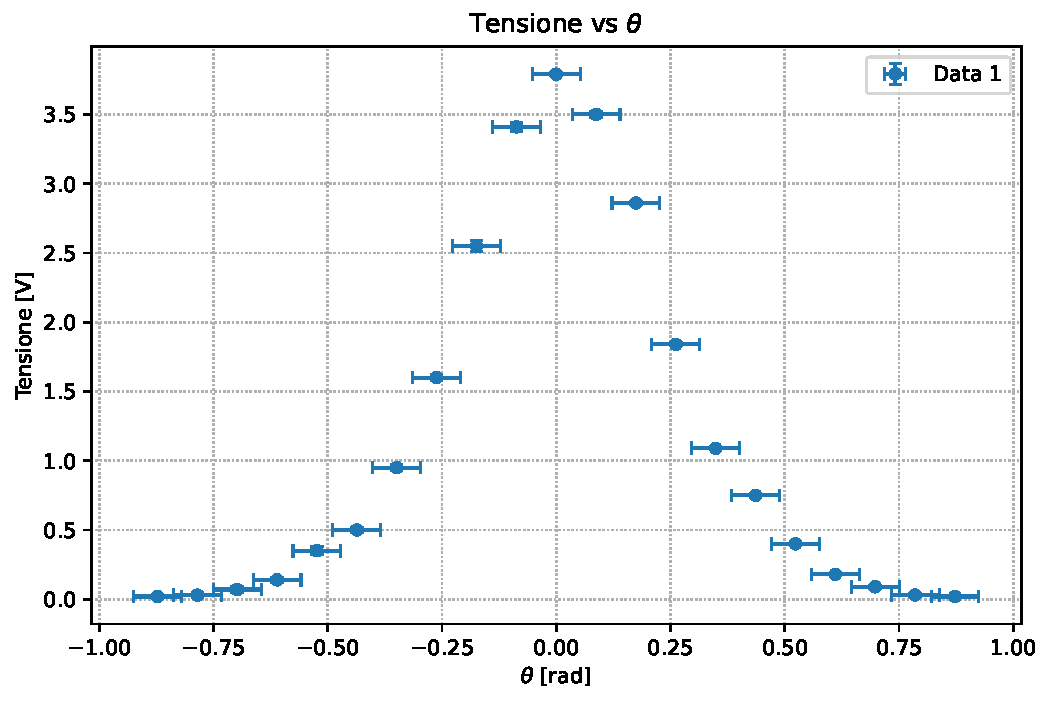
\includegraphics[width=0.8\textwidth]{grafici/theta_qualitativo.pdf}
	\caption{Grafico segnale - $\theta$.}
	\label{fig:theta_qualitativo}
\end{figure}
\textbf{Dipendenza del segnale dall'angolo $\theta$:}
I dati della \Cref{tab:dati_ampgeom_angolo}, riportati nel grafico in \Cref{fig:theta_qualitativo} mostrano che il segnale è massimo quando emettitore e ricevitore sono allineati ($\theta=0$) e decresce rapidamente all'aumentare dell'angolo $|\theta|$, indicando una significativa direzionalità del fascio. Per angoli superiori a circa $\SI{0.7}{\radian}$ ($\approx \ang{40}$), il segnale diventa molto piccolo. L'andamento appare qualitativamente simmetrico rispetto a $\theta=0$. Non è stato tentato un fit analitico specifico per questa dipendenza angolare.

\textbf{Onde stazionarie e stima della lunghezza d'onda $\lambda$:}
I dati in \Cref{tab:dati_ampgeom_ondestazionarie} mostrano chiare oscillazioni del segnale al variare della distanza $r$ su piccola scala. Queste oscillazioni sono dovute all'interferenza tra l'onda diretta e quelle riflesse tra emettitore e ricevitore, che formano onde stazionarie. La distanza tra due massimi (o minimi) consecutivi di questa figura di interferenza è pari a mezza lunghezza d'onda ($\lambda/2$).
Analizzando le posizioni dei massimi più evidenti nei dati (ad esempio, un massimo a circa $\SI{892}{\milli\metre}$ e un successivo a circa $\SI{879}{\milli\metre}$, oppure un massimo a $\SI{889}{\milli\metre}$ e un successivo a circa $\SI{876.5}{\milli\metre}$), si osserva una distanza tra massimi consecutivi di circa $\SI{12.5}{\milli\metre}$ a $\SI{13}{\milli\metre}$. Considerando una media di $\Delta r_{max} = \SI{12.75}{\milli\metre}$, e tenendo conto dell'incertezza di $\SI{1}{\milli\metre}$ su ogni misura di posizione (quindi circa $\SI{1.4}{\milli\metre}$ sulla differenza), si stima $\lambda/2 = \SI{12.75 \pm 1.4}{\milli\metre}$.
Da ciò si ricava la lunghezza d'onda:
$\lambda = 2 \times (\lambda/2) = 2 \times \SI{12.75 \pm 1.4}{\milli\metre} = \SI{25.5 \pm 2.8}{\milli\metre} = \SI{2.55 \pm 0.28}{\centi\metre}$.
Questo valore è compatibile con la lunghezza d'onda attesa di circa $\SI{3}{\centi\metre}$ (corrispondente a circa $\SI{10}{\giga\hertz}$) menzionata nell'introduzione al manuale.

\textbf{Andamento generale dell'ampiezza con la distanza $r$ (studio dei massimi):}
I dati in \Cref{tab:dati_ampgeom_massimi_distanza} mostrano che l'ampiezza del segnale (tensione misurata ai massimi delle onde stazionarie) aumenta al diminuire della distanza $r$. Se il fascio fosse un'onda sferica ideale e il ricevitore misurasse un segnale proporzionale all'ampiezza del campo elettrico, ci si aspetterebbe una dipendenza $V(r) \propto 1/r$.
È stato tentato un fit dei dati con un modello del tipo $V(r) = C + A/r$. I parametri ottenuti per $A$ e $C$ sono riportati nella \Cref{tab:risultati_fit_ampgeom_1_su_r}.

\begin{table}[htbp]
\centering
\begin{tabular}{|l|ccccc|}
\hline
Fit & A & C & $\chi^2$ & DoF & $\chi^2/\nu$ \\\hline\hline
Fit 1 (odr) & 1.542 ± 0.046 V/m & -998 ± 60 mV & 80.4 & 14 & 5.74 \\\hline
\end{tabular}
\caption{Risultati del fit dei dati di \Cref{tab:dati_ampgeom_massimi_distanza} con il modello $V(r) = C + A/r$.}
\label{tab:risultati_fit_ampgeom_1_su_r}
\end{table}

Il valore del $\chi^2/\nu = \num{5.74}$ per 14 gradi di libertà indica una scarsa compatibilità del modello con i dati sperimentali (p-value molto basso), il che suggerisce che il modello $A/r + C$ non è adeguato, o che vi sono problemi nella procedura di fit o nell'interpretazione dei parametri riportati.
Come indicato nel manuale di laboratorio, effetti al contorno, la natura non puntiforme della sorgente e del ricevitore (dovuta agli horn), e possibili riflessioni ambientali possono influenzare l'andamento del segnale, rendendo i modelli semplici inadeguati per una descrizione precisa.

\subsubsection{Conclusioni}
L'analisi dell'ampiezza e della geometria del fascio ha permesso di:
\begin{itemize}
    \item Confermare la natura direzionale del fascio di microonde, con il segnale che decade rapidamente allontanandosi dall'asse di emissione.
    \item Osservare chiaramente il fenomeno delle onde stazionarie dovute alle riflessioni multiple tra emettitore e ricevitore. Dall'analisi delle posizioni dei massimi e minimi di queste onde, è stato possibile stimare la lunghezza d'onda delle microonde, risultata pari a $\lambda = \SI{2.55 \pm 0.28}{\centi\metre}$. Questo valore è compatibile con quello atteso di circa $\SI{3}{\centi\metre}$.
    \item Studiare l'andamento dell'ampiezza del segnale (ai massimi delle onde stazionarie) in funzione della distanza $r$. Si osserva un aumento del segnale al diminuire di $r$. Tuttavia, un modello semplice di dipendenza $V(r) = C+A/r$ non descrive adeguatamente i dati, come indicato dal valore elevato del $\chi^2/\nu$ del fit e dalla problematica interpretazione dei parametri. Questa discrepanza è probabilmente dovuta alla complessità del sistema reale, che include la direttività degli horn, la loro prossimità, e possibili effetti di interferenza e diffrazione non modellizzati.
\end{itemize}


\section{Angolo di Brewster}
\subsection{Obiettivo}
Osservare come il fenomeno della rifrazione sia influenzato dalla polarizzazione dell'onda elettromagnetica incidente. Valutare la radiazione trasmessa attraverso la superficie di separazione tra due mezzi, al variare dell'angolo di incidenza, ottenendo una stima dell'angolo di Brewster caratteristico della rifrazione aria-polietilene. 

\subsection{Metodo}
Poiché avevamo a disposizione una sorgente d'onda polarizzata, ne abbiamo innanzitutto determinato la direzione di polarizzazione. Per fare ciò, è stata montata tra emettitore e ricevitore un'apposita griglia metallica e, variandone la posizione, è stata individuata la condizione tale per cui il segnale misurato risultava nullo, deducendo quindi informazioni sulla polarizzazione dell'onda in esame. Da tale osservazione abbiamo ricavato che disponendo emettitore, e quindi anche ricevitore, con il lato più corto parallelo al tavolo (configurazione~1) si aveva radiazione polarizzata parallelamente al piano di incidenza; viceversa, ruotando l'emettitore (configurazione~2) si otteneva un segnale con polarizzazione perpendicolare al piano di incidenza. Ci attendiamo quindi di poter determinare una stima dell'angolo di Brewster\footnote{Se un'onda polarizzata incide su una superficie di separazione tra due mezzi con polarizzazione parallela al piano di incidenza, l'intensità della radiazione riflessa e della radiazione trasmessa dipendono dall'angolo di incidenza. In particolare, in corrispondenza dell'angolo di Brewster, l'intensità dell'onda riflessa è nulla e, di conseguenza, quella dell'onda trasmessa è massima.} mediante l'utilizzo della prima configurazione.
Per osservare la variazione del segnale trasmesso correlata ad un diverso angolo di incidenza, abbiamo disposto sorgente e ricevitore frontalmente, a distanza fissa, e abbiamo ruotato gradualmente la lastra di polietilene posta tra i due. Ciò è stato possibile in quanto la lastra si poteva montare su di un goniometro che ne misurava quindi facilmente la rotazione. A tale rotazione corrispondeva una variazione dell'angolo di incidenza sia durante la rifrazione aria-polietilene (onda in entrata nella lastra) sia durante la rifrazione polietilene-aria (onda in uscita dalla lastra). L'informazione raccolta infatti dal ricevitore, e osservata sotto forma di tensione sul display del voltmetro, era correlata a un doppio fenomeno di rifrazione, tale per cui l'onda trasmessa ritornava in asse con l'onda incidente e quindi con la congiungente emettitore-ricevitore. 

\subsection{Dati}
Al fine di studiare l'intensità dell'onda trasmessa e la sua correlazione con l'angolo di incidenza, abbiamo misurato il segnale recepito dal ricevitore al variare dell'inclinazione della lastra di polietilene. Quest'ultima è stata ruotata di $\ang{5}$ alla volta. Il segnale osservato è stato misurato come tensione, quindi in volt. Gli angoli riportati corrispondono invece all'angolo formato dalla perpendicolare alla lastra con la direzione della radiazione incidente, diretta lungo l'asse emettitore-ricevitore. Per quanto riguarda la stima delle incertezze, abbiamo considerato fisso l'errore sull'angolo di incidenza, pari alla sensibilità del goniometro: $\delta_{\theta}=\ang{2}$. Per le tensioni, invece, abbiamo valutato come oscillava il segnale restituito dal voltmetro, ottenendo errori variabili, corrispondenti a metà dell'intervallo di oscillazione. Quanto misurato per ciascuna direzione di polarizzazione è riportato nelle \Cref{tab:brewster_par,tab:brewster_perp}.

\begin{table}[htbp]
\centering
\begin{tabular}{|c|c|}
\hline
$\theta$ & tensione \\\hline\hline
0 ± 30 mrad & 2.47 ± 0.01 V \\
87 ± 30 mrad & 2.46 ± 0.01 V \\
175 ± 30 mrad & 2.54 ± 0.01 V \\
262 ± 30 mrad & 2.59 ± 0.01 V \\
349 ± 30 mrad & 2.54 ± 0.01 V \\
436 ± 30 mrad & 2.55 ± 0.02 V \\
524 ± 30 mrad & 2.52 ± 0.01 V \\
611 ± 30 mrad & 2.68 ± 0.01 V \\
698 ± 30 mrad & 3.02 ± 0.01 V \\
785 ± 30 mrad & 3.62 ± 0.01 V \\
873 ± 30 mrad & 4.34 ± 0.01 V \\
960 ± 30 mrad & 4.66 ± 0.01 V \\
1.05 ± 0.03 rad & 4.45 ± 0.01 V \\
1.13 ± 0.03 rad & 3.00 ± 0.01 V \\
1.22 ± 0.03 rad & 1.58 ± 0.01 V \\
\hline
\end{tabular}
\caption{Dati di trasmissione con polarizzazione parallela al piano di incidenza.}
\label{tab:brewster_par}
\end{table}

\begin{table}[htbp]
\centering
\begin{tabular}{|c|c|}
\hline
$\theta$ & tensione \\\hline\hline
0 ± 30 mrad & 2.50 ± 0.01 V \\
87 ± 30 mrad & 2.55 ± 0.01 V \\
175 ± 30 mrad & 2.84 ± 0.01 V \\
262 ± 30 mrad & 2.90 ± 0.01 V \\
349 ± 30 mrad & 2.76 ± 0.01 V \\
436 ± 30 mrad & 2.66 ± 0.01 V \\
524 ± 30 mrad & 2.65 ± 0.01 V \\
611 ± 30 mrad & 2.52 ± 0.01 V \\
698 ± 30 mrad & 2.56 ± 0.01 V \\
785 ± 30 mrad & 2.71 ± 0.02 V \\
873 ± 30 mrad & 2.86 ± 0.02 V \\
960 ± 30 mrad & 3.17 ± 0.02 V \\
1.05 ± 0.03 rad & 2.64 ± 0.02 V \\
\hline
\end{tabular}
\caption{Dati di trasmissione con polarizzazione perpendicolare al piano di incidenza.}
\label{tab:brewster_perp}
\end{table}

\subsection{Analisi dati}
\begin{figure}[htbp]
	\centering
	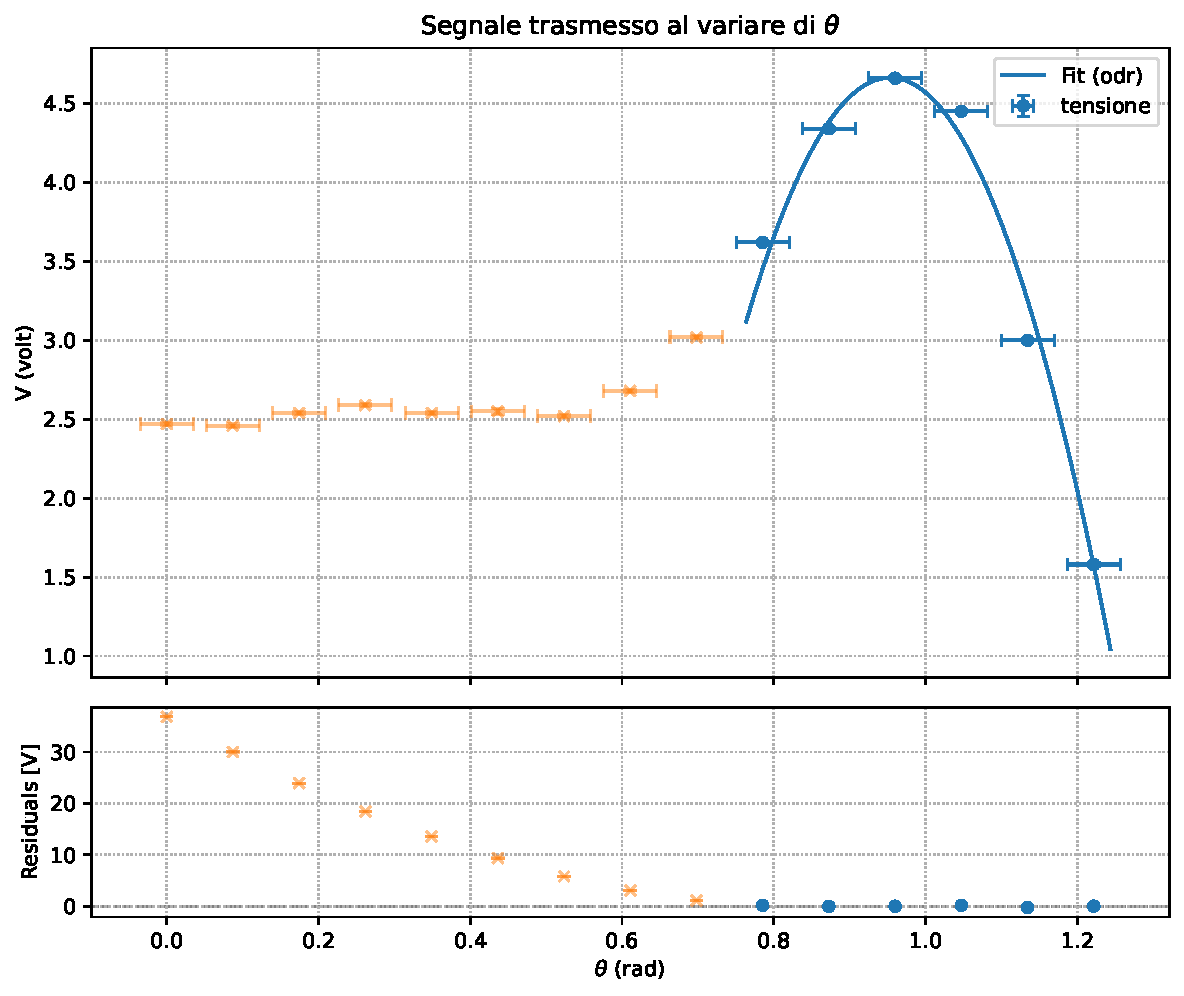
\includegraphics[width=0.8\textwidth]{grafici/brewster.pdf}
	\caption{Onda trasmessa con polarizzazione parallela al piano di incidenza.}
	\label{fig:brewster_par_grafico}
\end{figure}
\begin{figure}[htbp]
	\centering
	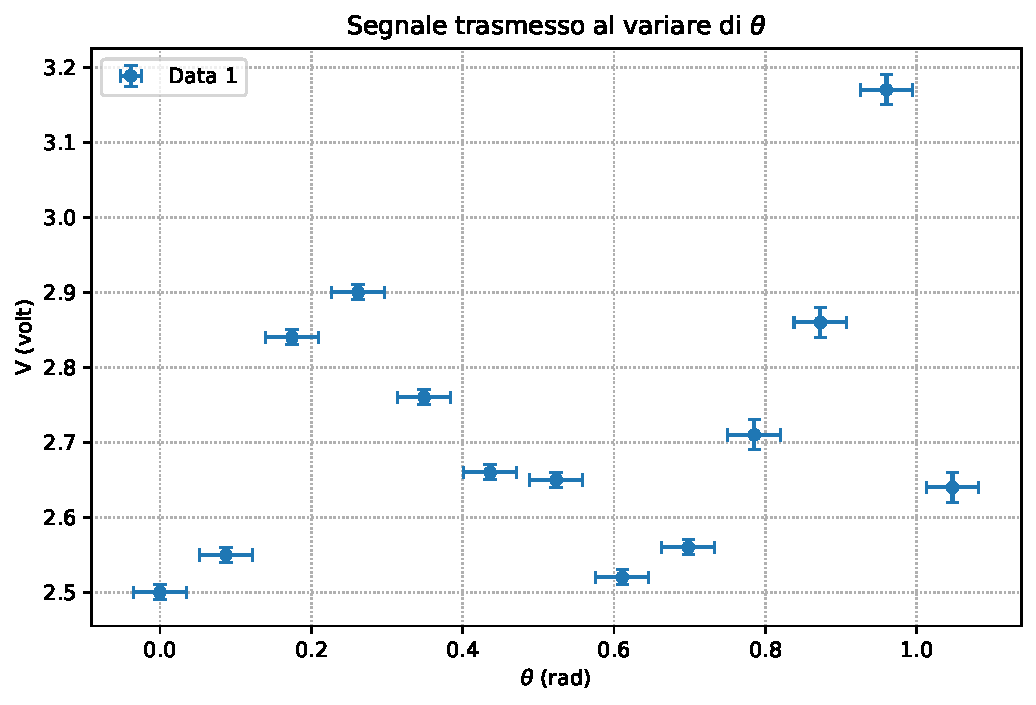
\includegraphics[width=0.8\textwidth]{grafici/brewster1.pdf}
	\caption{Onda trasmessa con polarizzazione perpendicolare al piano di incidenza.}
	\label{fig:brewster_perp_grafico}
\end{figure}

L'andamento del segnale ricevuto al variare di $\theta$ con polarizzazione parallela al piano di incidenza è visualizzabile nel grafico in \Cref{fig:brewster_par_grafico}. Il massimo del segnale trasmesso si ha in corrispondenza dell'angolo di Brewster, il cui valore è stato ottenuto attuando un'interpolazione parabolica sui punti campionati in prossimità del massimo. Si è utilizzata una relazione del tipo $y = ax^2 + bx +c$, con $y=V$ (tensione) e $x=\theta$ (angolo di incidenza), da cui si sono ricavati i parametri $a, b, c$ e i relativi errori, poi utilizzati per determinare la posizione del massimo. Più precisamente:
\begin{align}
  \theta_{B} = -\dfrac{b}{2a} \qquad & \text{e}\qquad
  \delta_{\theta_{B}} = \sqrt{\left(\dfrac{1}{2a}\delta_b\right)^2 + \left(\dfrac{b}{2a^2}\delta_a\right)^2}. \label{eq:angolo_brewster_calc}
\end{align}
Nella \Cref{tab:fit_brewster} sono raccolti i valori dei parametri di fit e la stima dell'angolo di Brewster.
\begin{table}[htbp]
\centering
\begin{tabular}{|l|ccccccc|}
\hline
Risultati & a & b & c & $\chi^2$ & DoF & $\chi^2/\nu$ & $\theta_B$ [\si{\degree}]\\\hline\hline
Fit Brewster & -42.9 ± 4.3 & 81.9 ± 8.4 & -34.4 ± 4.1 & 0.803 & 3 & 0.268 & 54.69 ± 7.84 \\\hline
\end{tabular}
\caption{Risultati del fit per la stima dell'angolo di Brewster.}
\label{tab:fit_brewster}
\end{table}
Per quanto riguarda invece le misurazioni effettuate con polarizzazione perpendicolare al piano di incidenza, come è possibile osservare dal grafico in \Cref{fig:brewster_perp_grafico}, si è osservato un segnale oscillante al variare di $\theta$. Inoltre, ponendosi più volte in corrispondenza dello stesso angolo si potevano misurare valori di tensione differenti. Abbiamo quindi interpretato quanto misurato come segnale di fondo. Tale ipotesi deriva anche dal fatto che le tensioni misurate con polarizzazione perpendicolare al piano di incidenza assumevano valori compresi tra $\SI{2.5}{\volt}$ e $\SI{3}{\volt}$, compatibili con il plateau iniziale rilevato per polarizzazione parallela al piano di incidenza.

\subsection{Conclusione}
Il valore dell'angolo di Brewster ricavato sperimentalmente, $\theta_B^{\text{sper}}$, è stato infine confrontato con quello atteso, $\theta_B^{\text{att}}$. Se si ha passaggio di un'onda elettromagnetica da un mezzo con indice di rifrazione minore ad uno con indice di rifrazione maggiore, come avviene durante l'ingresso dell'onda nella lastra, l'angolo di Brewster risulta pari a $\theta_B^{\text{att}} = \arctan\left(\frac{n_2}{n_1}\right)$, dove $n_1 = 1$ indica l'indice di rifrazione dell'aria, mentre $n_2 \approx 1.5$ corrisponde all'indice di rifrazione del polietilene. Il confronto tra $\theta_B^{\text{sper}}$ e $\theta_B^{\text{att}}$ è stato realizzato mediante z-test, con $z = \dfrac{|\theta_B^{\text{sper}} - \theta_B^{\text{att}}|}{\delta_{\theta_B^{\text{sper}}}}$. I suoi risultati sono riportati nella \Cref{tab:brewster_compatibilita}. Sebbene sia presente accordo tra quanto misurato e quanto atteso, è importante sottolineare che il segnale studiato non corrispondeva esattamente al segnale trasmesso in seguito al passaggio aria-polietilene, ma alla somma del segnale trasmesso per onda in entrata e in uscita dalla lastra di polietilene.
\begin{table}[htbp] 
\centering
\begin{tabular}{|l|c|}
\hline
$\theta_{att}$ [\si{\degree}] & Probabilità entro z sigma \\
\hline
56.31 & 0.58 \\
\bottomrule
\end{tabular}
\caption{Risultati del test di compatibilità tra $\theta_B^{\text{sper}}$ e $\theta_B^{\text{att}}$.}
\label{tab:brewster_compatibilita}
\end{table}


\section{Diffrazione di Bragg}
\subsection{Obiettivo}
\begin{figure}[htbp]
	\centering
	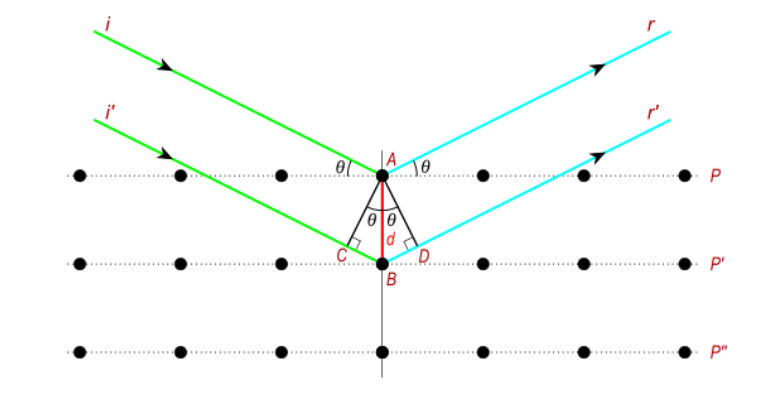
\includegraphics[width=0.5\textwidth]{grafici/schema.bragg.png}
	\caption{Schema del reticolo di Bragg.}
	\label{fig:schema_bragg}
\end{figure}

Verificare empiricamente la Legge di Bragg. Utilizzare un cubo realizzato in materiale plastico con incastonate all'interno sferette d'acciaio, atto a riprodurre in scala macroscopica la struttura reticolare di un cristallo. Studiare l'interferenza dovuta all'interazione tra i raggi riflessi dai diversi piani paralleli al piano reticolare (cioè dalle diverse file di sferette, come schematizzato in \Cref{fig:schema_bragg}) al variare dell'angolo $\theta$ di incidenza del fascio.

\subsection{Metodo}
\begin{figure}[htbp]
	\centering
	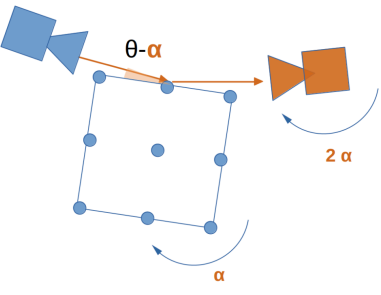
\includegraphics[width=0.4\textwidth]{grafici/disposizione.bragg.png}
	\caption{Disposizione dell'apparato sperimentale per la diffrazione di Bragg.}
	\label{fig:disposizione_bragg}
\end{figure}

Dopo aver posizionato il cubo di Bragg sul goniometro mediante l'utilizzo dell'apposito supporto, abbiamo disposto il ricevitore in modo tale che fosse possibile captare il segnale riflesso dal cubo. Per variare l'angolo di incidenza del fascio, abbiamo lasciato fisso l'emettitore e ruotato gradualmente il cubo. Ad ogni rotazione di un angolo $\alpha$ in senso orario del cubo seguiva una rotazione in senso orario di un angolo $2\alpha$ del ricevitore\footnote{Lo stesso ragionamento vale per rotazioni in senso antiorario.}, come si può osservare in \Cref{fig:disposizione_bragg}, in modo tale che il ricevitore puntasse nella direzione del raggio riflesso, dal momento che l'angolo di incidenza è uguale all'angolo di riflessione. Abbiamo quindi misurato il segnale acquisito dal ricevitore ad ogni rotazione. Tale procedura ci ha permesso però di osservare l'andamento del segnale soltanto parzialmente, in quanto siamo riusciti a campionare un numero limitato di angoli $\alpha$, poiché dovevamo mantenere una posizione reciproca tra ricevitore ed emettitore tale per cui il segnale prodotto non arrivasse direttamente al ricevitore senza prima incidere sul cubo.

\subsection{Dati}
Riportiamo nella \Cref{tab:dati_bragg} l'intensità del segnale misurato in corrispondenza degli angoli di rotazione considerati, definiti rispetto 
alla congiungente con l'emettitore.
Abbiamo stimato l'incertezza sul segnale, misurato come tensione, valutando l'oscillazione di quest'ultimo, scegliendo cioè come errore metà dell'intervallo di valori restituiti dal voltmetro. Per quanto riguarda invece l'incertezza sull'angolo di rotazione, abbiamo fissato $\delta_{\theta}=\ang{2}$, corrispondente all'angolo intercettato dalla punta del goniometro e cioè alla sensibilità dello strumento.

\begin{table}[htbp]
\centering
\begin{tabular}{|c|c|}
\hline
$\theta$ & tensione \\\hline\hline
349 ± 30 mrad & 30 ± 10 mV \\
401 ± 30 mrad & 30 ± 10 mV \\
436 ± 30 mrad & 30 ± 10 mV \\
471 ± 30 mrad & 40 ± 20 mV \\
524 ± 30 mrad & 90 ± 10 mV \\
559 ± 30 mrad & 180 ± 20 mV \\
611 ± 30 mrad & 210 ± 20 mV \\
663 ± 30 mrad & 230 ± 10 mV \\
698 ± 30 mrad & 280 ± 10 mV \\
750 ± 30 mrad & 320 ± 10 mV \\
785 ± 30 mrad & 300 ± 20 mV \\
838 ± 30 mrad & 150 ± 10 mV \\
873 ± 30 mrad & 140 ± 10 mV \\
960 ± 30 mrad & 20 ± 10 mV \\
1.05 ± 0.03 rad & 50 ± 10 mV \\
\hline
\end{tabular}
\caption{Dati sperimentali per la diffrazione dal cubo di Bragg.}
\label{tab:dati_bragg}
\end{table}

\subsection{Analisi dati}
\begin{figure}[htbp]
	\centering
	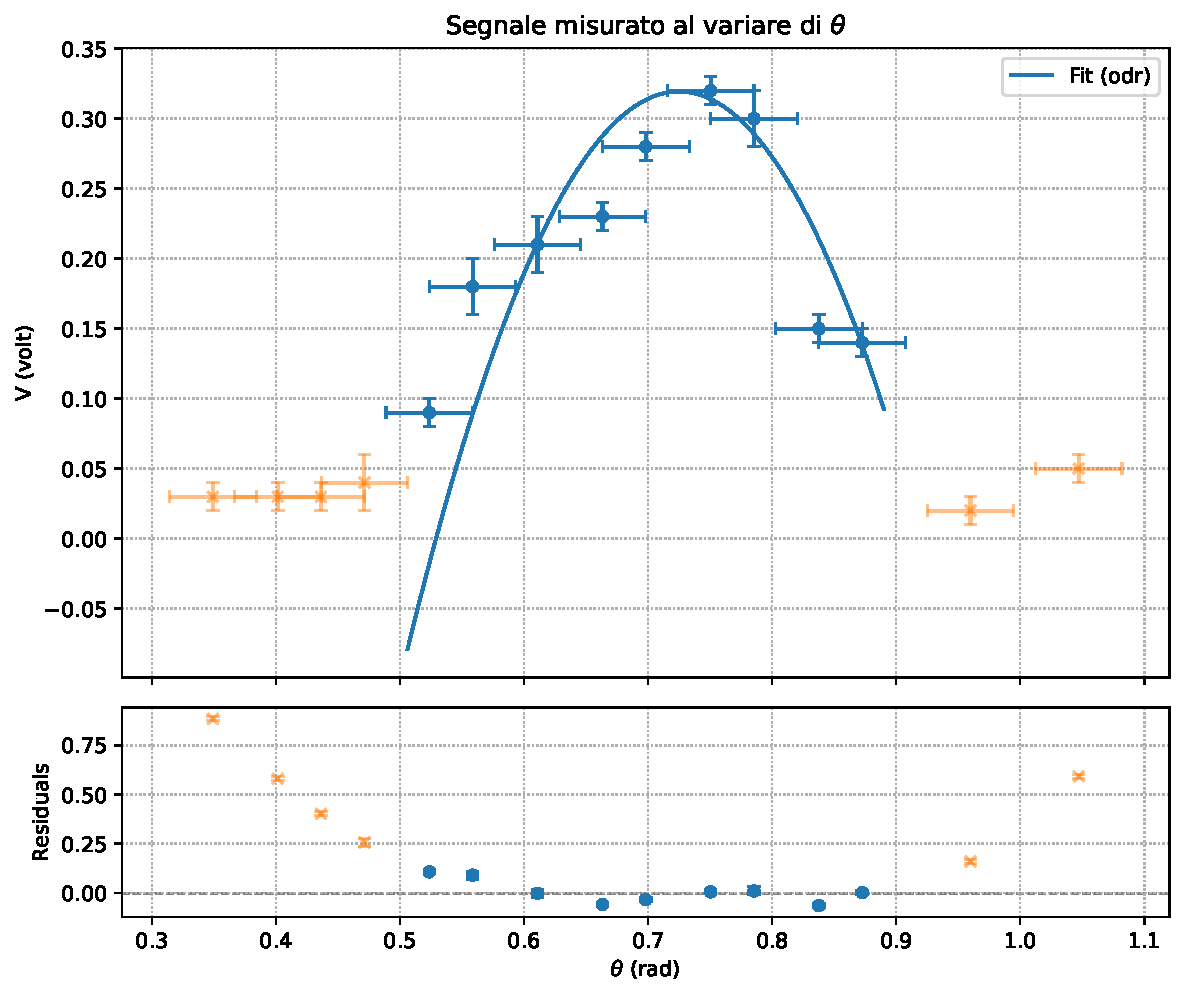
\includegraphics[width=0.8\textwidth]{grafici/bragg.pdf}
	\caption{Andamento del segnale misurato per la diffrazione dal cubo di Bragg.}
	\label{fig:grafico_bragg}
\end{figure}
La Legge di Bragg descrive la posizione dei massimi di interferenza, i quali si hanno in corrispondenza di $\theta$, angolo formato dal raggio incidente con il piano reticolare scelto, tale per cui vale la relazione:
\begin{align}
    n\lambda=2d \sin(\theta)
    \label{eq:legge_bragg} 
\end{align}
in cui $n$ indica l'ordine del massimo ed è quindi un numero intero, $\lambda$ è la lunghezza d'onda del raggio e $d$ corrisponde alla distanza tra due piani di sferette distinti. Nel caso in esame abbiamo misurato $d = \SI{3.8 +- 0.1}{\centi\metre}$.
Valutando l'andamento del segnale misurato al variare dell'angolo, visualizzabile in \Cref{fig:grafico_bragg}, abbiamo stimato la posizione del massimo di interferenza. Tale stima è stata ricavata utilizzando un'interpolazione parabolica applicata ai punti centrali del grafico. Abbiamo quindi utilizzato una legge della forma $y = ax^2 + bx +c$, con $y=V$ (tensione) e $x=\theta$ (angolo), a partire dalla quale abbiamo stimato i valori dei parametri $a, b, c$ e i relativi errori, poi utilizzati per ricavare la posizione del vertice. Più precisamente, abbiamo ricavato l'angolo per cui il segnale è massimo dalla relazione $\theta_{\text{max}} = -\dfrac{b}{2a}$, con errore $\delta_{\theta_{\text{max}}} = \sqrt{\left(\dfrac{1}{2a}\delta_b\right)^2 + \left(\dfrac{b}{2a^2}\delta_a\right)^2}$. Tale risultato ci ha permesso di ricavare la lunghezza d'onda della radiazione; invertendo la~\cref{eq:legge_bragg} e utilizzando la propagazione degli errori si ottiene\footnote{Si è ipotizzato di trovarsi in corrispondenza del primo massimo, cioè $n=1$.}:
\begin{align}
  \lambda_s = \dfrac{2d \sin(\theta_{\text{max}})}{n} \qquad & \text{e}\qquad
  \delta \lambda_s = \sqrt{\left( \dfrac{2d \cos(\theta_{\text{max}})}{n}\delta \theta_{\text{max}}\right)^2 + \left(\dfrac{2\sin(\theta_{\text{max}})}{n}\delta_d\right)^2}. \label{eq:lunghezza_bragg}
\end{align}
I risultati ricavati sono riportati nella \Cref{tab:fit_bragg}.
\begin{table}[htbp]
\centering
\begin{tabular}{|l|ccccccc|}
\hline
Risultati & a & b & c & $\chi^2$ & DoF & $\chi^2/\nu$ & $\lambda_s$ [\si{\meter}]  \\\hline\hline
Fit massimo & -8.3 ± 2.0 & 12.1 ± 2.8 & -4.0 ± 1.0 & 5.78 & 6 & 0.963 & 0.051 ±0.014\\\hline
\end{tabular}
\caption{Risultati del fit per la determinazione della lunghezza d'onda tramite la Legge di Bragg.}
\label{tab:fit_bragg}
\end{table}

\subsection{Conclusione}
Vogliamo sottolineare come l'andamento del segnale al variare dell'angolo non sia regolare, come è possibile osservare dalle misure riportate in \Cref{fig:grafico_bragg}. Tale irregolarità è da imputarsi agli effetti di bordo dovuti alla struttura di ricevitore e trasmettitore, ma anche ai vari fattori di rumore esterno, quali la presenza di dispositivi elettronici nei pressi della strumentazione o l'attività degli apparati sperimentali circostanti. Nel corso dell'esperienza abbiamo infatti potuto osservare come il segnale misurato dal voltmetro oscillasse anche a causa di fattori esterni. Ne consegue che abbiamo ottenuto una misura di $\lambda_s$ molto poco accurata, dal momento che presenta un errore relativo $\approx \SI{27}{\percent}$.

\end{document}
